%------------------------------------------------------------------------------
%	PACKAGES AND OTHER DOCUMENT CONFIGURATIONS
%------------------------------------------------------------------------------

\RequirePackage[l2tabu, orthodox, abort]{nag}
\documentclass[11pt, a4paper, openright, twoside]{memoir}

\chapterstyle{southall}

\checkandfixthelayout[nearest] % WHAT DOES THIS DO?

% Essentials
\usepackage[utf8x]{inputenc} % UTF8-support
\usepackage{ucs} % Extended UTF8-support
\usepackage[english]{babel} % Use english conventions in typesetting
\usepackage{fixltx2e} % Fixes some LaTeX stuff
\usepackage{graphicx, float} % Allows for graphics with fixed placement
\usepackage{booktabs} % Better tables
\usepackage{mathtools, amsmath, amsfonts, amssymb, amsthm} % Math-support

% Fonts
\usepackage{lmodern, tgpagella, eulervm}
\usepackage[T1]{fontenc}

% Customizable
\usepackage{subcaption}
\usepackage[dvipsnames]{xcolor}  % Coloured text etc.
\usepackage{tikz, tikzscale}
\usepackage{xifthen}
\usepackage{xargs}
\usepackage[colorinlistoftodos,prependcaption,textsize=footnotesize,%
obeyFinal,bordercolor=black,linecolor=black]{todonotes}
\usepackage[final]{pdfpages} % include pdfs
\usepackage{microtype}
\usepackage[bookmarks]{hyperref} % hyperlinks
\usepackage[nomain,acronym,xindy,toc,nonumberlist]{glossaries}
\usepackage{enumitem}
\usepackage{minted}

\usepackage[linesnumbered,noend,noline,boxed]{algorithm2e}
\usepackage[font={small,it},margin=.5cm]{caption}
\usepackage{etoolbox}
\AtBeginEnvironment{algorithm}{%
  \captionsetup{margin={-.5cm,.5cm}}%
}
\SetAlCapSkip{1.5ex}
\renewcommand\AlCapNameSty{\small\textit}
\renewcommand\AlCapSty{\small\textit}


% Keep here to make sure it loads last (but it is a "Essentials")
\usepackage[noabbrev,capitalize]{cleveref}

% Tikz styles
\tikzset{%
stein/.style 2 args={circle,inner sep=1pt,fill=white,draw,minimum size=5pt,label={#2:#1}},%
reg/.style 2 args={circle,inner sep=1pt,fill=black,minimum size=8pt,label={#2:#1}}%
}

% To-do commands
\newcommandx{\NOTE}[2][1=]{%
\todo[backgroundcolor=green!50,#1]{Note: #2}}

\newcommandx{\TODO}[2][1=]{%
\todo[backgroundcolor=yellow!50,#1]{ToDo: #2}}

\newcommandx{\FIXME}[2][1=]{%
\todo[backgroundcolor=red!50,#1]{FixMe: #2}}

\newcommandx{\missingref}[2][1=]{%
\todo[backgroundcolor=blue!50,#1]{Missing ref: #2}}

% Theorems, lemmas and corollaries
\newtheorem{theorem}{Theorem}[chapter]
\newtheorem{corollary}{Corollary}[theorem]
\newtheorem{lemma}[theorem]{Lemma}

% Hyperref setup
\hypersetup{
  bookmarks=true,
  colorlinks=true, % colored links
  linkcolor=red, % color of internal links
  citecolor=NavyBlue, % color of links to bibliography
  filecolor=cyan, % color of file links
  urlcolor=blue % color of external links
}

% Acronym setup
\renewcommand*{\glstextformat}[1]{\textcolor{black}{#1}}
\renewcommand*{\glsclearpage}{}
\makeglossaries{}
% Acronyms
\newacronym{smt}{SMT}{Steiner minimal tree}
\newacronym{rmt}{RMT}{relatively minimal tree}
\newacronym{estp}{ESTP}{euclidean Steiner tree problem}
% \newacronym{mst}{MST}{minimum spanning tree}
\newacronym{fst}{FST}{full Steiner tree}
\newacronym{fstp}{FST}{full Steiner topology}
% \newacronym{bnb}{BnB}{branch and bound}

%%% Local Variables:
%%% mode: latex
%%% TeX-master: "../main"
%%% End:


% Remove indent and use a line-skip instead
\nonzeroparskip{}
\setlength{\parindent}{0pt}

\newcommand{\chapterbreak}[0]{\par\fancybreak{$***$}\par}

%------------------------------------------------------------------------------
%	BEGIN DOCUMENT
%------------------------------------------------------------------------------

\pagestyle{ruled}

\begin{document}

%------------------------------------------------------------------------------
%	PRE-CONTENT - THESIS PAGES
%------------------------------------------------------------------------------

\frontmatter

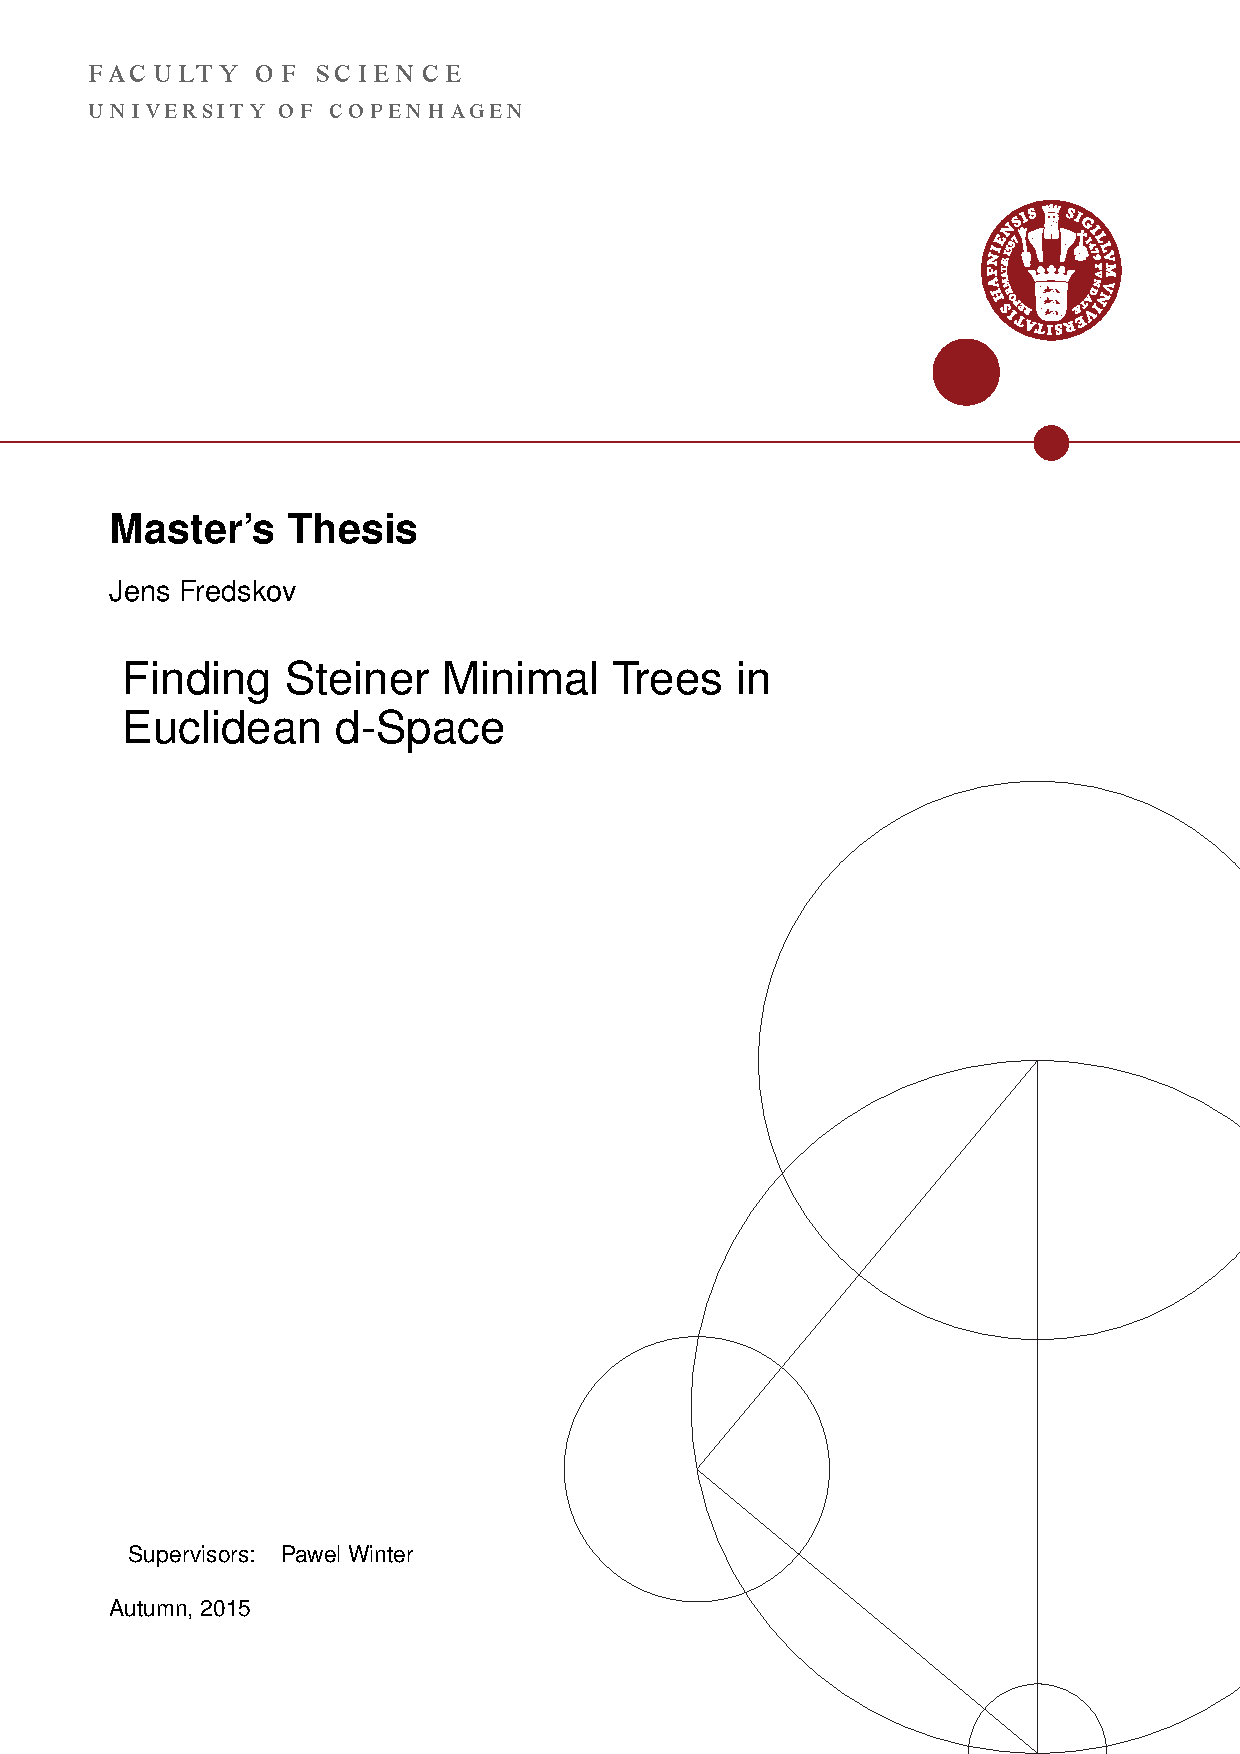
\includepdf{coverpage/coverpage}

\pagenumbering{roman} % Roman page numbering prior to the start of the thesis content (i, ii, iii, etc)

{
\abnormalparskip{0pt}
\chapter{Abstract}
\label{cha:abstract}
}

%%% Local Variables:
%%% mode: latex
%%% TeX-master: "../main"
%%% End:


{
\hypersetup{
  colorlinks=true, % colored links
  linkcolor=MidnightBlue, % color of internal links
}
\listoftodos{}
\tableofcontents
\listoftables
\listoffigures
\let\clearpage\relax
\printglossary[type=\acronymtype,title=Abbreviations]
}

%------------------------------------------------------------------------------
%	THESIS CONTENT - CHAPTERS
%------------------------------------------------------------------------------

\mainmatter

\pagenumbering{arabic} % Arabic page numbering for thesis content (1, 2, 3, etc)

{
\abnormalparskip{0pt}
\chapter{Introduction}
\label{cha:introduction}
}

% Introduction to the thesis

\section{Objectives}
\label{sec:objectives}

% The objectives

\section{Related work}
\label{sec:related-work}

2D: geosteiner, efficient algorithms for 2d

nD: smiths, smiths+, smiths*, other?

other: interesting versions of trees, rectilinear, or multiangle version

% Any related work

\section{Structural outline}
\label{sec:structural-outline}

% the overall outline of the thesis – each chapter and its contents

\chapterbreak{}

%%% Local Variables:
%%% mode: latex
%%% TeX-master: "../../main"
%%% End:

{
\abnormalparskip{0pt}
\chapter{Preliminaries}
\label{cha:preliminaries}
}

% Short introduction to the chapter (max 1/2 page)
The following chapter introduces basic concepts and definitions which either
help in understanding the problem area of the thesis, or which are directly used
by the thesis. The most important keywords of this chapter, which are directly
used in the thesis, are:
%
\begin{itemize}
\item Topologies and trees
\item Steiner trees: \aclp{fst}, \aclp{smt}
\item \aclp{estp}
\item Fermat-Torricelli point/problem
\end{itemize}
%
At the same time this chapter will introduce versions of the Steiner tree
problem which are not used directly by the thesis, but which help to give an
understanding of the problem area of the thesis, and which are mentioned in
\cref{cha:introduction} or discussed in \cref{cha:discussion}.

This chapter is mostly based on~\textcite{smith1992,gilbert1968,brazil2015} and
will by large follow the structure of~\cite[ch.~1]{brazil2015}.

\section{The Fermat-Torricelli Problem}
\label{sec:ferm-torr-probl}

Before introducing the Steiner problem, it is relevant to introduce the
Fermat-Torricelli problem, as this can be seen as a sort of subproblem to be
solved when solving the Steiner tree problem.

\newpage

The Fermat-Torricelli problem\footnote{The problem is so named as it was first
  proposed by \textcite{fermat1891} and the earliest known solution was put
  forth by \textcite{torricelli1919}.} in its classical two dimensonal form, is
defined as follows:
%
\begin{center}
\begin{tabular}{rp{9cm}}
  \toprule
  \textbf{Given} & A set of three points $V = \{p_1, p_2, p_3\}$ lying in the plane. \\
  \textbf{Find}  & A point $s$ such that the sum of the Euclidean distances from
                   $s$ to $p_1, p_2$ and $p_3$ is minimized. \\
  \bottomrule
\end{tabular}
\end{center}
%
The point $s$ will be referred to as a Steiner point\footnote{In the
  Fermat-Torricelli problem this point would normally be named the Fermat point
  or the Fermat-Torricelli point. However for clarity as to the connection
  between this problem and the Steiner problem this term is used. The name of
  both the Steiner problem/tree/point is named after Jakob Steiner, which might
  be errornous, who supposedly studied the Steiner problem for $3$
  terminals~\cite{brazil2014}.}. There are several ways to solve this problem,
e.g.\ using the rotation-proof~\cite[p.~3--5]{brazil2015}.

This formulation of the problem can be seen as a specialized instance of the
more general problem, where the edges are weighted. In the classical version the
weight of the edges are all equal to each other.

The generalized version for two dimensions of the problem can be formulated as in
\textcite{uteshev2014}:
%
\begin{center}
  \begin{tabular}{rp{9cm}}
    \toprule
    \textbf{Given} & Three non-colinear points $p_1 = (x_1, y_1)$, $p_2 = (x_2,
                     y_2)$ and $p_3 = (x_3, y_3)$ in the plane. \\
    \textbf{Find} & The point $p_\ast = (x_\ast, y_\ast)$ which gives a solution
                    to the optimization problem
                    \begin{gather}
                      \min_{(x,y)} \sum_{j=1}^3 m_j \sqrt{{(x-x_j)}^2 + {(y-y_j)}^2}
                    \end{gather}
    Where the weight of $j$th point, $m_j$, is a real positive number. \\
    \bottomrule
  \end{tabular}
\end{center}
%
The generalized Fermat-Torricelli problem can be even further generalized from
two dimensions to $d$ dimensions, with $d \ge 2$
\cite{fermattorricelliproblem}. This simply requires the points to be
$d$-dimensional and the optimization problem to be changed to the following:
%
\begin{gather}
  \min_{(x_1, x_2, \ldots, x_d)} \sum_{j=1}^3 m_j
  \sqrt{\sum_{i=1}^d {(x_i - x_{(j,i)})}^2 }
  \\ \Updownarrow \\
  \label{eq:4}
  \min_{(p)} \sum_{j=1}^3 m_j | p p_j |, \quad p \in \mathbb{R}^d
\end{gather}
%
Solving the Fermat-Torricelli problem with even weights is equivalent with solving
the smallest possible instance of the \acl{estp}. The analytical solution
presented by~\textcite{uteshev2014} and a generalization of it to $\mathbb{R}^d$ is
presented in \cref{sec:analyt-solut-ferm}.

\section{The Euclidean Steiner Tree Problem}
\label{sec:eucl-stein-tree}

We firstly define a graph $G = (V(G), E(G))$ where the vertices $V(G)$ are
points of the graph, $V(G) \subset \mathbb{R}^d$ and the edges
$E(G) \subset (\mathbb{Z}^{+} \times \mathbb{Z}^{+})$ are straight lines
connecting the points in $V(G)$. The euclidean length of edge $e \in E(G)$ we
denote $|e|$.

The \ac{estp} is then defined as follows:
%
\begin{center}
  \begin{tabular}{rp{9cm}}
    \toprule
    \textbf{Given} & A set of points $R = \{ p_1, p_2, \ldots, p_n \}$ in
                     $\mathbb{R}^d$. \\
    \textbf{Find} & A graph $T = (V(T), E(T))$ such that $R \subseteq V(T)$, and
                    $|T| = \sum_{e \in E(T)} |e|$ is minimized. \\
    \bottomrule
  \end{tabular}
\end{center}
%
Note that $T$ must be a tree, as any cycles can obviously be removed without
disconnecting the graph or increasing the length. An example of the difference
between the \ac{mst} and \ac{smt} can be seen in \cref{fig:points-mst-smt}.
%
\begin{figure}[htbp]
  \centering
  \includegraphics[width=0.5\textwidth]{gfx/tikz/points-mst-smt}
  \caption[\acs{mst} vs. \acs{smt}]{Example of the difference between the \acs{mst} (left)
    and \acs{smt} (right) for the three points $p_1 = (0,0), p_2 = (0, 2), p_3 = (2,
    1)$. The \acs{mst} simply interconnects the existing points with the shortest
    possible tree. The \acs{smt} however adds an extra point $s_4 = (0.577, 1)$
    and interconnect these four points with the shortest possible tree. The is
    not way to interconnect the three original points with a shorter tree, no
    matter the number of extra points we add than in the left
    tree.\label{fig:points-mst-smt}}
\end{figure}

\section{Steiner Minimal Tree}
\label{sec:steiner-minimal-tree}

We define a \ac{smt} as in \textcite{brazil2015}, which is as follows:
%
\begin{definition}[\acl{smt}, Steiner points, terminals]
  A tree $T = (V(T), E(T))$ representing a solution to the Steiner tree problem
  is called a \acl{smt}. The given points $R \subseteq V(T)$ are called
  terminals and possible extra vertices $S = V(T) \setminus R$ are called
  Steiner points.
\end{definition}
%
The definition used by \textcite{smith1992} is simply that a \ac{smt} on $n$
terminals is the shortest tree containing the terminals. This definition, while being
a bit more convoluted, is essentially the same as the one given by
\textcite{brazil2015}. Thus we use that definition as it is more verbose and
gives a definition of Steiner points and terminals as well.

\section{Topologies}
\label{sec:topologies-1}

A topology is the combinatorial structure of a tree, or other form of geometric
network. This means that in a topology only the adjacencies of points
matter. Thus we could represent the topology of the tree $G = (V(G), E(G))$ as
just the edges of the tree $E(G)$ and any graph (and tree) has an
underlying topology.

We call any tree of some topology non-degenerate if all edges of the tree have
non-zero length---otherwise the tree is called degenerate.

We now define a Steiner topology and a full Steiner topology as the following:
%
\begin{definition}[Steiner topology, full Steiner topology]
The topology of a non-degenerate \ac{smt} is called a Steiner topology. The
topology of a non-degenerate \ac{smt} in which every terminal has degree 1 is
called a full Steiner topology.
\end{definition}
%
Notice that a full Steiner topology must necessarily have the most possible
Steiner points so $ k = n - 2$. This can be seen by substituting $n_2 = n_3 = 0$
and $n_1 = n$ in \cref{eq:22}.

\section{Steiner Trees}
\label{sec:steiner-trees}

Before defining Steiner trees we define \acp{rmt} as in~\cite{gilbert1968}
as:
%
\begin{definition}[\acl{rmt}]
  A tree is called a \acl{rmt} if it is the shortest possible tree of its
  underlying topology.
\end{definition}
%
As can easily be seen a \ac{smt} must also be a \ac{rmt} of its underlying
topology. Finally we define Steiner trees. Steiner trees currently have two
definitions which are not exactly identical.

The first is the definition used by \textcite{gilbert1968}, combined with the
definition for \acp{fst} in \textcite{smith1992}, is as follows:
%
\begin{definition}[Steiner tree, \acl{fst}]
  If a tree can be shortened no further even when splitting is allowed, the tree
  is called a Steiner tree. If all of the original points\footnote{I.e.\ the
    points not inserted when splitting. These are what we have so far referred
    to as the terminals.} of a Steiner tree have degree 1 the tree is called a
  \acl{fst}.\label{def:steiner-tree}
\end{definition}
%
Here the process of splitting referred to is exactly what we do when e.g.\
inserting an extra point in the Fermat-Torricelli problem. Thus it follows
pretty straightforward that a Steiner tree must also be a \ac{rmt} of the
topology which describes it\footnote{Note that here we refer to the topology we
  end up with after we cannot split any more points, and not the topology we
  started out with.}. Furthermore any \ac{smt} must also be a Steiner tree, but
not vice versa as illustrated by \cref{fig:steiner-smts}.
%
\begin{figure}[htbp]
\centering
\includegraphics[width=0.6\textwidth]{gfx/tikz/steiner-smts}
\caption[Example of splitting and \acsp{rmt}]{Example of how of splitting a point
  and inserting a new Steiner point. The flow shows two of the paths splitting
  could take on the shown topology down until no more splitting is
  possible. Optimizing the two final topologies, both are obviously \acsp{rmt} of
  their underlying topology, but only the right one is a \acs{smt} as the other
  topology is degenerate (the two Steiner points lie on top of each other in the
  center). Thus if the original points are the terminals, only the last right
  tree is a \acs{smt} for the original terminals.\label{fig:steiner-smts}}
\end{figure}
%
The other, and newer definition, used by \textcite{brazil2015} is as follows:
%
\begin{definition}[Steiner tree, \acl{fst}]
  A non-degenerate (full) \ac{rmt} for a Steiner topology is called a (full)
  Steiner tree.\label{def:steiner-tree2}
\end{definition}
%
These definitions are not exactly identical as e.g.\ the last tree to the left
in \cref{fig:steiner-smts} would not be a Steiner tree by
\cref{def:steiner-tree2}\footnote{As it has an edge of length zero.}  but would
be by \cref{def:steiner-tree}. The similarities of the two definitions should
however be obvious, and it also holds for both of the definitions that any
\ac{smt} must be a Steiner tree, and that any Steiner tree must be a \ac{rmt} of
its underlying topology. The one we will use in general is
\cref{def:steiner-tree2}.

Finally there is also the definition used by
\textcite{smith1992}, which defines a Steiner tree, by some properties which it
must also have for it to satisfy the above definitions. This is as follows
%
\begin{definition}[Steiner tree]
\leavevmode\vspace{-\baselineskip}\par
\begin{enumerate}
\item It contains $n$ terminals
  $R = \{ p_1, p_2, \ldots, p_n \} \in \mathbb{R}^d$, and possibly $k$
  additional Steiner points
  $S = \{ p_{n+1}, \ldots, p_{n+k} \} \in \mathbb{R}^d$.
\item Each Steiner point has degree $3$, the edges emanating from it are
  coplanar and have a mutual angles of $120^{\circ}$.
\item Each terminal has degree at most $3$.
\item $0 \le k \le n-2$.
\end{enumerate}
\end{definition}
%
\begin{proof}
The first property is by definition, to name the terminals and the
Steiner points.

The second and third property can be shown in the following way: First consider
that any Steiner point must have at least degree $3$. This should be obvious as
a Steiner point with degree $1$ does not connect any terminals to the rest of
the tree, and thus the point can simply be removed to either shorten the tree or
keep it the same\footnote{Which could happen if a Steiner point was lying atop
  the point is connected to.}. Furthermore every Steiner point with a degree of
$2$ can be removed, and its edges be replaced with one edge that is of the same
length or shorter as per the Triangle Inequality
Theorem\cite{triangleinequality}.

We now show that no pair of edges emanating from a Steiner point can have a
mutual angle less than $120^{\circ}$. This can be proven in a few different
ways. The one used by \textcite{gilbert1968} is based on the mechanical model
presented described in the same article. A simpler approach in my own opinion
however is the one used by \textcite{brazil2015}. The proof is follows: Consider
a point $a$ in $T$, and a pair of non-zero edges $ab, ac \in E(T)$ meeting at
$a$. Note that $ab$ and $ac$ must form a shortest interconnection of the points
$\{a, b, c\}$ and furthermore we know that a solution the Fermat-Torricelli
problem for $\{ a, b, c \}$ forms a shortest interconnection as well. An
immediate consequence\footnote{This stems from the fact that the
  Fermat-Torricelli problem has a solution at one of the points if any of the
  angles is greater than $2 \pi / 3$ and somewhere between them otherwise. The
  details can either be found in \textcite[ch.~1]{brazil2015} or somewhat
  implicitly in \cref{sec:analyt-solut-ferm}.} of this is that the angle between
$ab$ and $ac$, denoted $\angle bac$ must be at least $2 \pi / 3 = 120^{\circ}$.
To see that this is true, assume that it is smaller; We then have two cases as
shown in \cref{fig:preliminaries-steiner-point} and in neither cases is $ab$ and
$ac$ a shortest interconnection of $\{a, b, c\}$.

\begin{figure}[htbp]
\centering
\includegraphics[width=0.6\textwidth]{gfx/tikz/preliminaries-steiner-points}
\caption[Obtaining shorter trees]{Replacing a pair of edges $ab$ and $ac$ for
  which $\angle bac < 2 \pi / 3$ with a shortest interconnection provided by a
  solution to the Fermat-Torricelli problem for $\{a,b,c\}$. The left figure has
  no angle greater than $120^{\circ}$. The right has a angle $\angle cba \ge
  120^{\circ}$. In both cases a shorter tree is constructed. This figure is the
  same as in
  \textcite[p.~7]{brazil2015}.\label{fig:preliminaries-steiner-point}}
\end{figure}

Using that the mutual angles may be no less than $120^{\circ}$ it follows that
any point in $T$ can have at most degree $3$\footnote{As
  $3 \cdot 120^{\circ} = 360^{\circ}$ meaning that there is at most room for
  three edges around a point.}. It therefore follows that terminals have a
degree of at most $3$, which proves the third property, and that Steiner points
have a degree of exactly $3$ and thus also mutual angles of precisely
$120^{\circ}$, proving the second property.

The fourth property follows in the following way from property 3 and 4. Any tree
$T$ has $|V(T)|-1$ edges. Thus a Steiner tree has $n+k-1$ edges.  Every edge has
two endpoints meaning there are $2 n + 2 k - 2$ edges. As every Steiner point
has a degree of $3$, they account for $3 k$ of the endpoints. For the terminals
we must split them in three groups: $n_1$, those that have a degree of
$1$. $n_2$, those that have a degree of $2$ and, $n_3$, those that have a degree
of $3$. The terminals thus account for the rest of the endpoints, written as
$n_1 + 2 n_2 + 3 n_3 \ge n$. We can then write the equation as
%
\begin{align}
  \label{eq:22}
  3 k + n_1 + 2 n_2 + 3 n_3 &= 2 n + 2 k - 2 \\
  k &= 2 n - 2 - (n_1 + 2 n_2 + 3 n_3) \\
  0 \le k &\le n - 2
\end{align}
%
Thus proving the fourth property.
\end{proof}

\section{Finding Steiner Trees in 2D}
\label{sec:find-stein-trees-2}

In general the problem of finding \acp{smt} is NP-hard. This however is only a
measure of the worst-case upper bound. Thus in some cases it may indeed be
possible to find them much faster.

In two dimensions algorithms exists, which in many cases can find the \acp{smt} much
faster than the worst-case scenario.

This section will give a short introduction to the Hwang-Melzak and GeoSteiner
algorithm. Afterwards the section will discuss why these algorithms do not
generalize to dimensions higher than two.

\subsection{The Hwang-Melzak Algorithm}
\label{sec:hwang-melz-algor}

The Hwang-Melzak algorithm was first presented by \textcite{melzak1961} and
later improved by \textcite{hwang1986hexagonal}. For a proof of correctness see
\textcite{hwang1986linear, melzak1961}.

The algorithm is used for optimizing the tree $T$ of a pre-specified full
Steiner topology $\mathcal{T}$ with at least $n \ge 5$ terminals, assuming that
$T$ is non-degenerate. The algorithm can be implemented to run in
$\mathcal{O}(n)$. The algorithm is very well-known, and is also presented in
\textcite{brazil2015,smith1992}.

Before describing the algorithm, we define an equilateral point.
%
\begin{definition}{Equilateral point}
  An equilateral point $e_{ab}$, of the points $a$ and $b$, is a point such that the
  triangle $\triangle a b e_{ab}$ is equilateral. It is clear that in two dimensions
  such a point has two unique placements, one on each side of the line passing
  through $a$ and $b$.
\end{definition}
%
The algorithm consists of two steps. The first, the \textit{merging} step, works
as follows: Let $u$ be a Steiner point connected to $a$, $b$ and $s$, where $a$
and $b$ are terminals\footnote{It can be proven, that such a pair can always be
found. However intuitively it also makes sense, by simply thinking about the
number of terminals and Steiner points in a full Steiner topology, and realizing
that no Steiner point can be connected solely to other Steiner points, and thus
we must be able to find such a point.}. Replace $a$, $b$ and $u$ with a the
equilateral point $e_{ab}$ of $a$ and $b$. Do this $n-2$ times until the
topology consists of only $2$ points. The second step, the
\textit{reconstruction} step, works a follows: Let $\mathcal{T}'$ be the full
Steiner topology on the $n-1$ new terminals\footnote{I.e.\ the same set of
  terminals as before, but where $a$ and $b$ has been replace with
  $e_{ab}$}. Then the coordinates of $u$ can be found by taking the intersection
between the Steiner arc $\widehat{ab}$\footnote{The arc between $a$ and $b$ on the
  circle circumscribing the triangle $\triangle a b e_{ab}$.} and the edge
$e_{ab}s$. Do this on the $2$ point tree $n-2$, reinserting the points
represented by the equilateral points, until we again have a tree of $n$
terminals with the correct coordinates for the $n-2$ Steiner points.

It may well be that $\widehat{ab}$ and $e_{ab}s$ do not intersect, if this is
the case, the algorithm halts, and no solution exists for the given full
Steiner topology.

The biggest issue of the above algorithm is deciding on which side of the line
$ab$ we should place the equilateral point $e_{ab}$. However it turns out that
by choosing the order in which we perform the merging steps we are always able
to find the correct side. Thus this algorithm runs in $\mathcal{O}(n)$.

\NOTE[inline]{If time add a more detailed description of how we decide side of
  equilateral point, and add a figure of the two steps of Hwang-Melzak.}

The proof of the algorithm and how to decide the side for the equilateral point
can be found in \textcite[ch.~1]{brazil2015}.

The algorithm unfortunately does not generalize from two dimensions to higher
dimensions. The reason for this is, that while the edges emanating from a
Steiner point are indeed coplanar, the plane the points lie in is not known in
advance if there are more than $3$ terminals. This means that we no longer have
a unique pair of equilateral points for each cherry\footnote{A pair of terminals
  adjacent to a common Steiner point in a Steiner topology is called a cherry
  for the topology.}, but instead a continuous range of equilateral points lying
on a circle in $d$-space, as illustrated by \cref{fig:equi-points}.
%
\begin{figure}[htbp]
  \centering
  \begin{subfigure}[t]{0.4\textwidth}
    \includegraphics[width=\textwidth]{gfx/tikz/equi-points-2d}
    \caption{When $d = 2$ we have exactly two unique possible
      placements.\label{fig:equi-points-2d}}
  \end{subfigure}\\hspace{1em}%
  \begin{subfigure}[t]{0.4\textwidth}
    \includegraphics[width=\textwidth]{gfx/tikz/equi-points-3d}
    \caption{When $d \ge 3$ we have a circle in $d$-space of possible
      placements. Here $d = 3$ is shown.\label{fig:equi-points-3d}}
  \end{subfigure}
  \caption[Equilateral points in 2D and $d$-space]{The case where $d = 2$ only
    has the two unique possible placements of the equilateral point $e_{ab}$ for the
    two points $a$ and $b$, one of which can be eliminated when running the
    algorithm. However when $d \ge 3$ this is no longer the case, and we are
    unable to determine a unique placement of the equilateral
    point.\label{fig:equi-points}}
\end{figure}
%
Thus in contrast to the two dimensional case where we can select one of the two
unique equilateral points, in higher dimensions we are no longer able to do
this, and the algorithm breaks down.

\subsection{The GeoSteiner Algorithm}
\label{sec:geosteiner-algorithm}

\NOTE[inline]{if time add figure.}

The GeoSteiner algorithm was originally proposed by \textcite{winter1985}. Later
improvements of the implementation have allowed for the computation of \acp{smt}
for several thousand terminals~\cite{brazil2015}.

The GeoSteiner algorithm is pretty involved, and will thus not be described in
greater detail here. In general the algorithm has two phases. In the first
(\textit{generation}) phase, \acp{fst} for all full Steiner topologies of all
subsets of terminals are generated. This enumeration can be said to be done
implicitly\footnote{as opposed to explicitly defining each \ac{fst} one at a
  time.} by simulating the Hwang-Melzak algorithm, and using geometric
properties to prune parts of the Steiner arcs on which the Steiner points can
lie. In this way the algorithm can prune \acp{fst} of full Steiner which cannot
be part of the final \ac{smt}, and if all \acp{fst} of a full Steiner topology
is pruned, i.e.\ if no feasible part of a Steiner arc is left, the entire full
Steiner topology can be pruned. The strength of the algorithm lies partly in
generating \acp{fst} with similar full Steiner topologies in a single pass and
partly in being able to prune partially constructed full Steiner topologies. In
the second, (\textit{concatenation}) phase, the algorithm selects a subset of
not pruned \acp{fst} that span all terminals and has the minimum total
length. This concatenation can be formulated as the minimum spanning tree
problem in a hypergraph, which is indeed also NP-hard. However using a
branch-and-cut algorithm most instances can be solved quite
effectively\footnote{For an implementation of GeoSteiner see e.g.\
  \url{http://www.diku.dk/hjemmesider/ansatte/martinz/geosteiner/}.}. For a
fuller description of the algorithm, see e.g.\ \textcite[sec.~1.4]{brazil2015}.

While the algorithm is the most effective currently known for $d = 2$, it is
unfortunately not applicable when $d \ge 3$. First, the generation of \acp{fst}
for all subsets of terminals in $\mathbb{R}^d, d \ge 3$, is much more difficult
than in $\mathbb{R}^2$. Optimizing a \ac{fst} with more than $3$ terminals when
$d \ge 3$ requires solving high-degree polynomials~\cite{smith1992}. As a
consequence of this we can never use a algorithm such as Hwang-Melzak, but must
use numerical approaches, such as \citeauthor{smith1992}'s optimization routine
described in \cref{cha:algorithm}. Such numerical approaches seem to block the
generation of \acp{fst} across various subsets of terminals. Furthermore many of
the geometrical properties used to prune seems to be much weaker when
$d \ge 3$~\cite{fonseca2014}.

Finally \textcite[p.~142]{smith1992} describes, that it seems when $d \ge 3$,
that the topology of a \ac{smt} often consists of only a single large \ac{fst}
involving all $n-2$ Steiner points, instead of many small edge-disjoint
\acp{fst}. Whether this is true, is not really qualified by
\textcite{smith1992}, but it does seem likely that the \acp{fst} will tend to
grow larger when we get to higher dimensions, as we have more space in which
the Steiner point can lie. Thus we will not be able to leverage the benefits of
the two phases in GeoSteiner, as the \acp{fst} we generate in the first phase
will span a large portion of the set terminals, or possibly even the entire
set, making that phase very large and the second phase trivial.

\section{Finding Steiner Trees in $d$-Space}
\label{sec:find-stein-trees-d}

As described in \cref{sec:geosteiner-algorithm} determining \acp{fst} in
$\mathbb{R}^d, d \ge 3$ requires solving high-degree polynomials, and thus we
need to resort to numerical approaches.

The most well-known of these is \citeauthor{smith1992}'s algorithm, proposed by
\textcite{smith1992}. This algorithm is described in much greater detail in
\cref{cha:algorithm}, but in general it works by enumerating all full Steiner
topologies and then optimize these using an iteration which
converges to the \ac{fst} of that full Steiner topology. The algorithm can be
implemented with a branch-and-bound approach\footnote{The approach is not
  completely classic branch-and-bound as we are only able to bound, after having
  generated a complete solution. We do however generate small sub-problems of
  fewer terminals, and using the found bounds are able to prune these and their
  entire tree descendants/solutions. Thus in this way the algorithm can indeed
  be seen as branch-and-bound. The details of this can be found in
  \cref{cha:algorithm}.}, such that the found \acp{fst} can be used to prune
full Steiner topologies before optimizing them. The algorithm however cannot
solve problem instances with more than around $15$ to $20$ terminals within a
feasible amount of time.

There have been several attempts at optimizing \citeauthor{smith1992}'s
algorithm to improve its speed and thus increase the number of terminals
feasible to solve. Some of these are

\begin{itemize}
\item \textcite{fampa2008} proposed using lower bounds on partial Steiner
  topologies\footnote{I.e.\ topologies that do not include all $n$ terminals.}
  to prune \acp{fst}. Roughly the method works in the following way: Imagine we
  have a \ac{fst} not connecting all $n$ terminals. To select the next terminal
  to connect to the topology we compute the lower bounds
  $z^{\ast}(\bar{D}_l^{+})$ of every terminal not yet connected, and select the
  terminal for which the largest number of descending topologies can be
  pruned. In this way the lower bound allow \citeauthor{fampa2008} to both prune
  some descendants of topologies, and also vary the order in which they connect
  terminals to reduce the number of topologies they need to optimize. The conic
  formulation and the actual lower bound will not be discussed here as they are
  rather extensive. The method shows some improvement on both the number of
  topologies enumerated and the actual running time. However as pointed out by
  \textcite{fonseca2014} while a smaller number of \acp{fst} are generated,
  the time spent on computations increase significantly, and thus the speed
  gained from computing these lower bounds is minimal when compared to e.g.\
  distance-based sorting of the terminals.
\item \textcite{vanlaarhoven2013} proposed both a method for sorting the
  terminals by their distance to the centroid and a set of geometric criteria
  used to prune non-optimal \acp{fst}. The use of geometric criteria is partly
  what makes the 2D algorithms so successful, and thus it seems natural to
  explore these for the $d$-space case as well. However again as noted by
  \textcite{fonseca2014} these computations give very little when compared to
  simply sorting the terminals based on distance in terms of speed vs.\ time
  spent on computations.
\item \textcite{fonseca2014} proposed a way of sorting the terminals, such that
  the first three terminals maximized the sum of their pairwise distance, and
  all terminals afterwards maximize the sum of their distances to the already
  spanned terminals.
\end{itemize}

\NOTE[inline]{If time, add
  \url{http://www.iasi.cnr.it/aussois/web/uploads/2015/papers/fampam.pdf}}

Finally \textcite{fonseca2014} has also proposed a new branch enumeration
algorithm, instead of \citeauthor{smith1992}'s algorithm. This algorithm draws
its inspiration from the GeoSteiner algorithm. Instead of enumerating full Steiner
topologies and optimizing their respective trees it creates branches of subsets
of terminals. The algorithm utilizes that upon removed a Steiner point from a
full Steiner topology, $3$ branches are created, and that one can always find a
Steiner point, such that the branches have at most $\lfloor \frac{n}{2} \rfloor$
terminals, which reduces the number of branches that need to be generated. The
algorithm then consists of three phases. First, it computes \acp{smt} for subsets
with up to $8$ terminals. Second, it generates branches containing up to
$\lfloor \frac{n}{2} \rfloor$ terminals, and the \acp{smt} found in the first
phase are used to prune away branches that cannot be part of the final
\ac{smt}. Finally it generates full Steiner topologies with $n$ terminals by
concatenating three disjoint branches. The shortest tree found is then
outputted. \citeauthor{fonseca2014} noted that the branch enumeration algorithm
was able to solve many of the tested topologies with $15$ terminals within the
given time of 12 hours which \citeauthor{smith1992}'s, even with terminal
sorting, was not.

There has also been some work into heuristics and approximation algorithms. This
is however somewhat limited, and out of scope for this thesis as we here mainly
focus on \citeauthor{smith1992}'s algorithm and exact algorithms.

\section{Variations on the Steiner Tree Problem and Applications}
\label{sec:vari-stein-tree}

Steiner trees can of course be modified in several different ways. One could
think of changing both the metric, the constraints, the cost function and so
on. Some of the more well-known, are presented here with reference to where one
could read more about the type of Steiner tree if so desired. The section also
discuss some of the real world applications of Steiner trees, i.e.\ their
usefulness outside the academic world as more than a mathematical curiosity.

Some of the types of Steiner trees to mention are:
%
\begin{itemize}
\item \textbf{Rectilinear Steiner Tree} \quad A version of the Steiner tree in which
  edges must consist of vertical and horizontal line segments. It can be proven,
  that an edge always only needs to consist of at most a single horizontal, and
  a single vertical line segment, and thus we calculate the edge length using
  the rectilinear $\mathcal{L}_1$ norm. See e.g.~\textcite[ch.~3]{brazil2015}.
\item \textbf{Fixed Orientation Steiner Tree} \quad A version the of Steiner tree,
  which can be seen as a generalization of the rectilinear Steiner tree. In this
  version the metric used is a fixed orientation metric, meaning that edges are
  only allowed to have some fixed orientations, the rectilinear version can be
  seen as a fixed orientation version where we have two perpendicular
  orientations. See e.g.~\textcite[ch.~2]{brazil2015}.
\end{itemize}
%
Of possible applications, some more mentionable are:
%
\begin{itemize}
\item \textbf{Electronic circuits/VLSI Design} \quad Both rectilinear and fixed
  orientation Steiner trees have use in VLSI design and the realization of
  electronic circuits as described by
  \textcite[sec.~2.7,sec~3.6]{brazil2015}. When designing electronic circuits
  the wires between components can normally only be drawn in a rectilinear, or
  lately fixed orientation, matter. Thus Steiner trees can be used to pack the
  components closer. This also has uses for higher dimensions than $2$. As
  electronic components normally consists of several layers in which the wires
  can run between, thus crossing each other without shorting, the problem also
  has use in $3$ dimensions.
\item \textbf{Phylogenetics} \quad A method using $d$-space Euclidean Steiner trees
  has been proposed to be used in the determination of phylogenetic trees by
  \textcite{brazil2009}. Phylogenetic trees are used to determine the
  relationship between different species, these are represented as the leafs of
  the tree, and the interior nodes are then their ancestors. In this way one can
  represent the genetic difference of species, as their distance in the
  phylogenetic tree.
\end{itemize}
%
\textcite{brazil2015} cover several more possible variations on Steiner trees,
and applications of Steiner trees for the interested reader.

\NOTE[inline]{If time add obstacle-avoiding Steiner trees and possible uses for
  these in applications.}

%%% Local Variables:
%%% mode: latex
%%% TeX-master: "../../main"
%%% End:

\chapter{Smiths algorithm}
\label{ch:algorithm}

% Short introduction to the chapter (max 1/2 page)
The following chapter will describe the different parts of the algorithm used by
Smith~\cite{Smith1992}. \TODO{Finish introduction}

\section{Overview}
\label{sec:overview}

The algorithm in general follow the form of as proposed by Gilbert and
Pollak~\missingref{18 in Smith}

\TODO[inline]{Finish the overview}

\TODO[inline]{Add a note that while there may not have been other ways to go at
  the time, today we also have things such as the one described in Fonseca,
  Pawel, et al.}

\section{Topologies}
\label{sec:topologies}

The first step of the algorithm is, as described in \Cref{sec:overview}, to
generate topologies. It is therefore natural that we need some way of
representing and generating these topologies.

The algorithm only considers full Steiner topologies where $K = N - 2$. This is
a \NOTE{is there a better word than legal?} legal approach as we can simply
regard any Steiner tree with $K \le N - 2$ as a \ac{FST} where some edges have
length zero and thus some points have ``merged''.

\subsection{Representation}
\label{sec:representation}

\begin{figure}[htbp]
\centering
  \begin{subfigure}[b]{0.3\textwidth}
    \includegraphics[width=\textwidth]{gfx/tikz/algorithm-topology-1}
    \caption{Here be dragons.\label{fig:algorithm-topology-1}}
  \end{subfigure}
~
  \begin{subfigure}[b]{0.3\textwidth}
    \includegraphics[width=\textwidth]{gfx/tikz/algorithm-topology-2}
    \caption{Here be dragons.\label{fig:algorithm-topology-2}}
  \end{subfigure}
~
  \begin{subfigure}[b]{0.3\textwidth}
    \includegraphics[width=\textwidth]{gfx/tikz/algorithm-topology-3}
    \caption{Here be dragons.\label{fig:algorithm-topology-3}}
  \end{subfigure}
\caption[How to construct Steiner topologies]{Here be dragons.\label{fig:algorithm-topologies}}
\end{figure}

There is an 1--1 correspondence between full Steiner topologies with $N \ge 3$
regular points, and $(N-3)$-vectors $\vec{a}$, whose $i$th entry $a_i$ is an
integer between $1 \le a_i \le 2 i + 1$.

\TODO[inline]{Describe/Outline proof and the generation as shown in the figures.}

\subsection{Generation}
\label{sec:generation}

Using the representation described in \Cref{sec:representation} the problem of
generating all topologies can now be done as a backtracking problem generating
all $(N-3)$-topology vectors.

\TODO[inline]{Describe the backtracking here}

To further speed up the generation of topologies, or rather to avoid generating
unnecessary topologies, Smith also utilizes the following theorem

\begin{theorem}
For any set of $N$ distinct regular points in any Euclidean space, the length of
the shortest tree, interconnecting $N-1$ points, with topology vector $a_1
\cdots a_{N-4}$ is no greater than the length of the shortest tree,
interconnecting $N$ points, with topology vector $a_1 \cdots a_{N-3}$.
\end{theorem}

\TODO[inline]{Proof of above theorem}

The algorithm utilizes this to prune in the following way. Imagine we have found
some upper bound for the \ac{SMT}. If we then optimize any generated topology
vector which does not yet include all the regular points, and it turns out to
have length greater than the upper bound, we can prune any topologies that we
would have generated from this vector, as the length of the larger topologies
cannot become any smaller than the length of the current, and thus cannot become
smaller than the length of the upper bound.

Thus the implementation of the algorithm generates and optimizes topologies
depth-first to ensure we get a upper bound as quickly as possible. If it did
breadth-first we would not be able to prune anything, as we would get all the
full topologies as the last to optimize.

\section{Optimization of a topology}
\label{sec:optim-topol}

\TODO[inline]{TODO}

\subsection{Iteration}
\label{sec:iter-fixm-could}

\FIXME[inline]{This section could probably be better named}
\TODO[inline]{TODO}

%%% Local Variables:
%%% mode: latex
%%% TeX-master: "../../main"
%%% End:

 {
\abnormalparskip{0pt}
\chapter{Implementation}
\label{cha:implementation}
}

The new implementation has been written in the, still relatively new but at this
point stable, language Go, which quoting the homepage: ``Go is an open source
programming language that makes it easy to build simple, reliable, and efficient
software.''~\cite{golanghomepage}. Go is a general-purpose, strongly typed and
garbage-collected language. The syntax bears resemblance to C\footnote{But
  with a lot less braces, and no pointer arithmetic.}. Furthermore Go has
explicit support for concurrent programming. The language furthermore sports
extremely fast compiling of source code and tries to have performance
comparable to C.

The reasoning behind choosing Go for the new implementation were firstly that I
already had experience with the language making it easy to get to work on the
new implementation without also having to learn a new programming
language. Secondly the language has, in my opinion, a very clean syntax which
makes it easily readable for anyone familiar with any C-syntax styled
language. Finally the easy use of concurrency in Go\footnote{Starting a new
  goroutine, which is the languages type of lightweight threads, is as simple as
  writing: \texttt{go~SomeFunction~(args\ldots)}.} made it interesting as
continued work with the new implementation could include a potential,
significant, speedup by making the branching of the algorithm concurrent. The
same could be be true for the Gauss elimination, concurrent\footnote{Not
  concurrency has actually been implemented in the new implementation. However
  the possibilities of this is discussed in \cref{sec:concurrency}.}.

In general the implementation tries to follow guidelines given in
\textcite{effectivego}. These are guidelines as to how one codes effective
Go. Here effective means both in terms of speed, memory usage, stability and
readability.

Source code for the new implementation, fixes for the old implementation and
experiments can be found at \url{https://github.com/jsfr/SteinerExact}. The
source code for just the new implementation is also included in
\cref{cha:source-code}.

This chapter will describe the architecture of the new implementation, i.e.\ how
the new implementation has been structured.

\TODO[inline]{Describe the source code architecture, and rewrite introduction so
it makes sense with new structure.}

\section{Main and Config File}
\label{sec:main-file}

\section{\acs{smt} Package}
\label{sec:smt-package}

\subsection{Data Structures}
\label{sec:data-structures}

\subsection{Methods}
\label{sec:methods}

%%% Local Variables:
%%% mode: latex
%%% TeX-master: "../../main"
%%% End:

{
\abnormalparskip{0pt}
\chapter{Benchmarks and Tests}
\label{cha:benchmarks-tests}
}

\chapterbreak{}

%%% Local Variables:
%%% mode: latex
%%% TeX-master: "../../main"
%%% End:

{
\abnormalparskip{0pt}
\chapter{Discussion}
\label{cha:discussion}
}

\endChapter{}

%%% Local Variables:
%%% mode: latex
%%% TeX-master: "../../main"
%%% End:

{
\abnormalparskip{0pt}
\chapter{Conclusion}
\label{cha:conclusion}
}

\chapterbreak{}

%%% Local Variables:
%%% mode: latex
%%% TeX-master: "../../main"
%%% End:


%------------------------------------------------------------------------------
%	POST-CONTENT  - APPENDIX AND BIBLIOGRAPHY
%------------------------------------------------------------------------------

\backmatter

\appendix

\label{app:bibliography}
\bibliographystyle{ieeetr}
\bibliography{content/backmatter/bibliography}

% \chapter{Source Code}
\label{cha:source-code}

\newmintedfile[golang]{go}{
  frame=lines,
  framesep=2mm,
  fontsize=\footnotesize,
  linenos,
  tabsize=4,
  baselinestretch=0.8,
}

\golang[label=point.go]{sourcecode/smt/point.go}
\golang[label=edge.go]{sourcecode/smt/edge.go}
\golang[label=helpers.go]{sourcecode/smt/helpers.go}
\golang[label=tree.go]{sourcecode/smt/tree.go}
\golang[label=optimize.go]{sourcecode/smt/optimize.go}
\golang[label=main.go]{sourcecode/main.go}

%%% Local Variables:
%%% mode: latex
%%% TeX-master: "../../main"
%%% End:


\end{document}

%%% Local Variables:
%%% mode: latex
%%% TeX-master: t
%%% End:
